\documentclass[letterpaper]{article}

\usepackage{underscore}
\usepackage[left=2.0cm, right=2.0cm, top=2.0cm]{geometry}
\usepackage[utf8]{inputenc}
\usepackage{graphicx}
\usepackage{graphics}
\usepackage[spanish]{babel}
\usepackage{lipsum}
\usepackage{float}
\usepackage{subfigure}
\title{EV\_1\_1\_circuitos\_de\_rectificación\_no\_controlados}
\author{Ledesma Hernández Miguel Ángel y Alcantar Díaz Joel Alejandro}
\date{17/09/2019}

\begin{document}
{\maketitle}






\vspace{6cm}
\begin{center}
    \textbf{Universidad Politécnica  de la Zona Metropolitana de Guadalajara}\\

\end{center}



\vspace{.3cm}
\begin{center}
\centering

\includegraphics[scale=0.3]{UPZMGLog.png}\\
\vspace{1cm}

    \textbf{Mecatr\'onica 4to A: Sistemas electr\'onicos de interfaz}

\end{center}

\newpage










    \begin{LARGE}
            \textbf{Objetivos:}\\
    \end{LARGE}
    %aqui escribe los objetivos de la práctica en una frase pequeña \lipsum[1-2] es la madre de lorem
         \begin{large}
           \\ Crear circuitos de rectificacion y obserbar la onda generada por los mismos.

         \end{large}
\vspace{2cm}
    
    
    
    
    
    
    
    
    
        \begin{LARGE}
            \textbf{Materiales:}\\
         \end{LARGE}
    \begin{large}
      \begin{table}[htbt]
      \centering
      \begin{tabular}{|l|l|l|}
      \hline
      \multicolumn{3}{|c|}{Materiales}\\ \hline
      Componentes & Equipo & Programas\\
      \hline \hline
          No utilizados & Computadora & Orcad o Kicad\\ \hline
      \end{tabular}
      
      \end{table}
            
    \end{large}
    \vspace{1.2cm}
    
    
         \begin{LARGE}
            \textbf{Procedimientos:}\\
         \end{LARGE}
         
         
         
         
         
         
    \begin{large}
        Se creara un nuevo proyecto de Orcad para cada circuito representado en la practica.
        \begin{enumerate}
            \item Se selecciona en el menu superior File - New - Project... como se muestra en la figura 1\\
            \begin{figure}[htb]
                \centering
                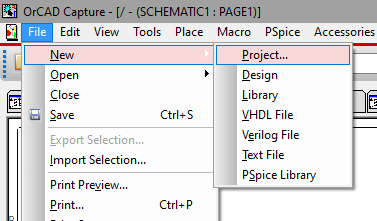
\includegraphics[scale=1]{p1.png}
                \caption{Menu de creacion}
                \label{fig:Menu Creacion}
            \end{figure}
            \item Se nombra al proyecto y se selecciona 'Analog or mixed A/D' y despues 'OK' como en la figura 2\\ \newpage
            \begin{figure}[htb]
                \centering
                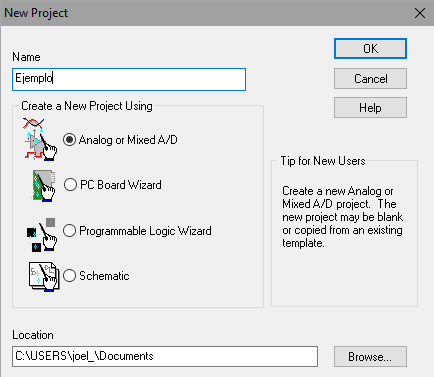
\includegraphics[scale=0.5]{p2.png}
                \caption{Primera pantalla del menu 'New Project'}
                \label{fig:Menu New project}
            \end{figure}
            \item Aparecera una nueva ventana como la de la figura 3 en la que se marcara la opcion 'Create a blank project' y se selecciona 'Ok'\\
            \begin{figure}[htb]
                \centering
                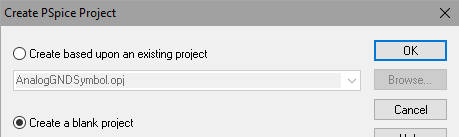
\includegraphics[scale=0.6]{p3.png}
                \caption{Ventana de creacion de proyecto PSpice}
                \label{fig:Creacion PSpice}
            \end{figure}
        \end{enumerate}
        Con el proyecto ya creado se procede a elaborar el circuito y para ello se seguiran los pasos a continuacion descritos.
        \begin{enumerate}
            \item En la secci\'on 'Place part' se activara el filtro de compatibilidad con PSpice como se muestra en la figura 4. De esta manera solo trabajaremos con piesas compatibles con PSpice.\\
            \begin{figure}[htbp]
                \centering
                \subfigure[Identificacion de las opciones]{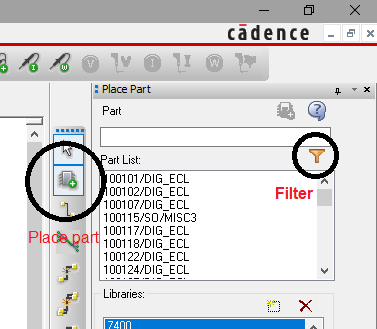
\includegraphics[scale=0.7]{cp1.png}}
                \subfigure[Opciones de filtrado]{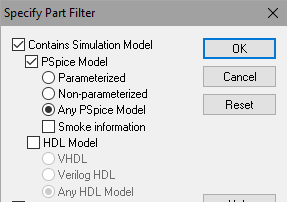
\includegraphics[scale=0.7]{fil.png}}
                \caption{Configuracion de filtrado}
                \label{fig:Configuracion de filtro}
            \end{figure} \newpage
            \item Se busca el componente que se requiere en la seccion 'Part'como se muestra en la figura 5 ahora con la seguridad de que es compatible con PSpice.\\
            \begin{figure}[htbp]
                \centering
                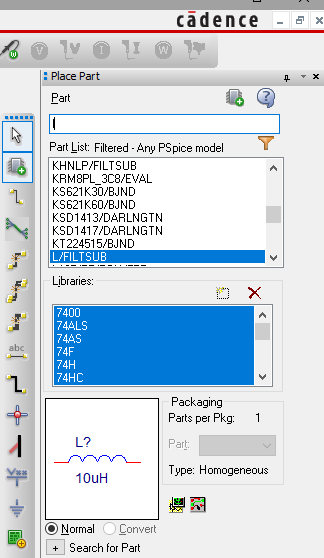
\includegraphics[scale=0.5]{cp2.png}
                \caption{Busqueda de parte}
                \label{fig:Busqueda de parte}
            \end{figure}
        \end{enumerate}
        Se debera tomar la tierra mostrada en la figura 6.\newpage
        \begin{figure}[htbp]
            \centering
            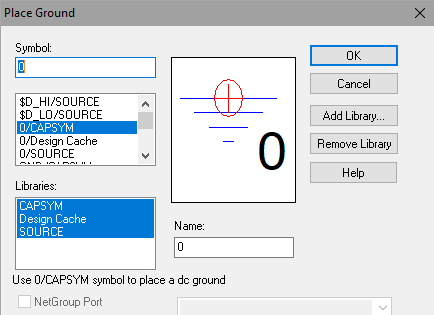
\includegraphics[scale=0.5]{gnd.png}
            \caption{Tierra para la simulacion}
            \label{fig:GNDsim}
        \end{figure}
        Se procede a armar el circuito siguiendo el esquema de la pagina 10 del documento como se muestra en la figura 7.\\ Los componentes para este circuito son:\\
        \begin{enumerate}
            \item Alternador (VSIN).
            \item Diodo ideal (Dbreak).
            \item Bobina (L)
            \item Resistencia (R)
        \end{enumerate}
        \begin{figure}[htbp]
        \centering
        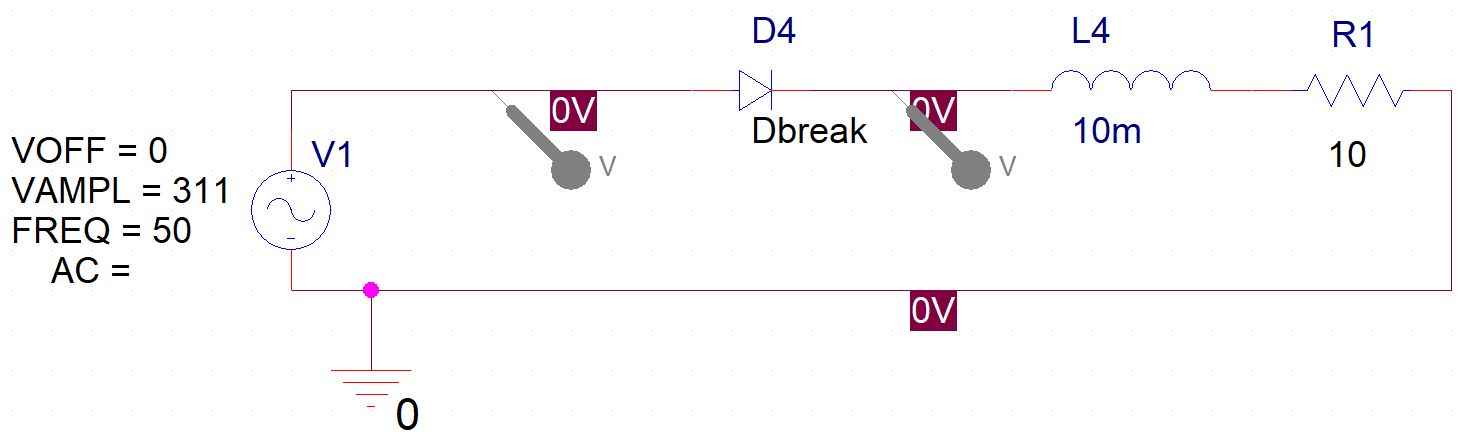
\includegraphics[scale=0.4]{cir1.png}
        \caption{Circuito pagina 10.}
        \end{figure}
        Se sigue armando los circuitos siguiendo los esquemas presentados en la practica.
        \begin{figure}
            \centering
            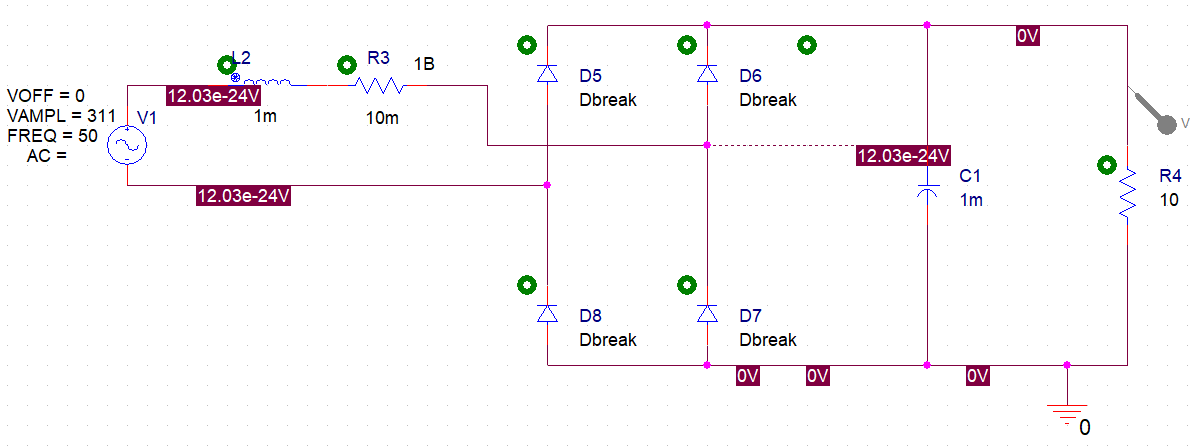
\includegraphics[scale=0.5]{cirp13y22.png}
            \caption{Circuito pagina 13 y 22.}
            \label{fig:Cir13y24}
        \end{figure}\newpage
        \begin{figure}[htbp]
            \centering
            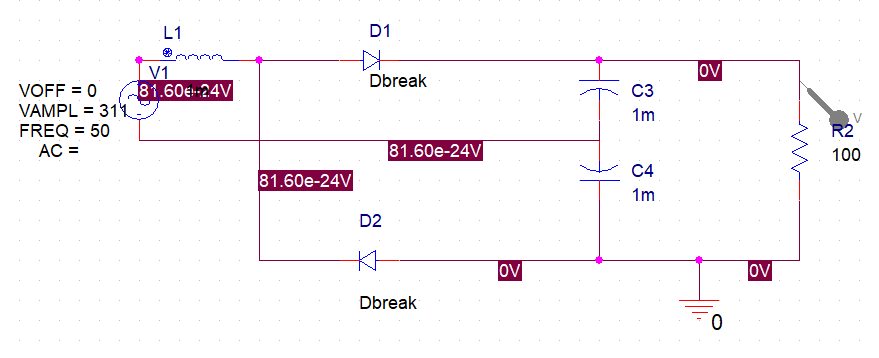
\includegraphics[scale=0.8]{cirp25.png}
            \caption{Circuito página 25}
            \label{fig:Cirp25}
        \end{figure}\newpage
        Para la realizacion del circuito de la pagina 28 primero se tiene que elaborar la simulacion del circuito de la pagina 29, posteriormente conectarlos como detalla en el esquema de la pagina 28.
        \begin{figure}[htbp]
            \centering
            \subfigure[Circuto de la pagina 29.]{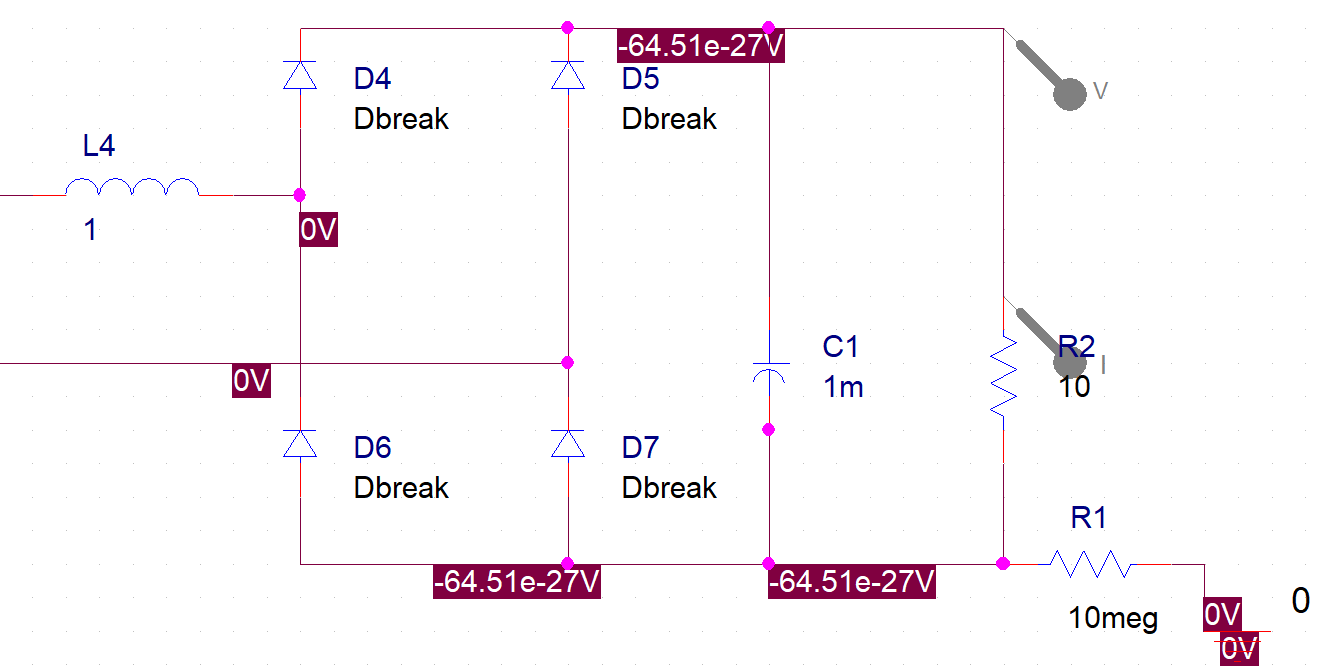
\includegraphics[scale=0.4]{cirp29.png}}
            \subfigure[Circuito pagina 28.]{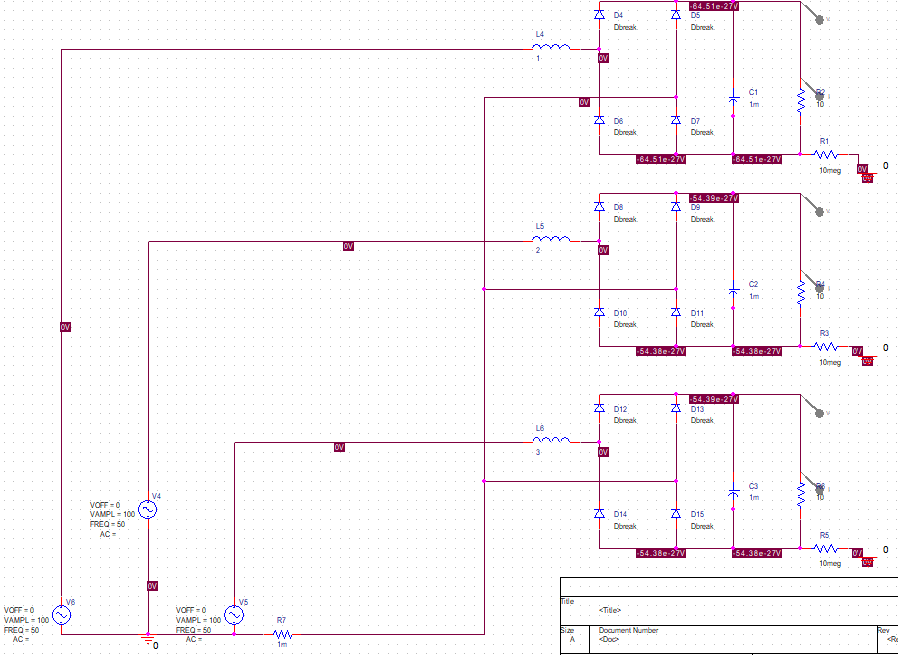
\includegraphics[scale=0.4]{cirp28.png}}
            \caption{Circuitos complementarios pagina 28 y 29.}
            \label{fig:cirp28y29}
        \end{figure}
        \begin{figure}[htbp]
            \centering
            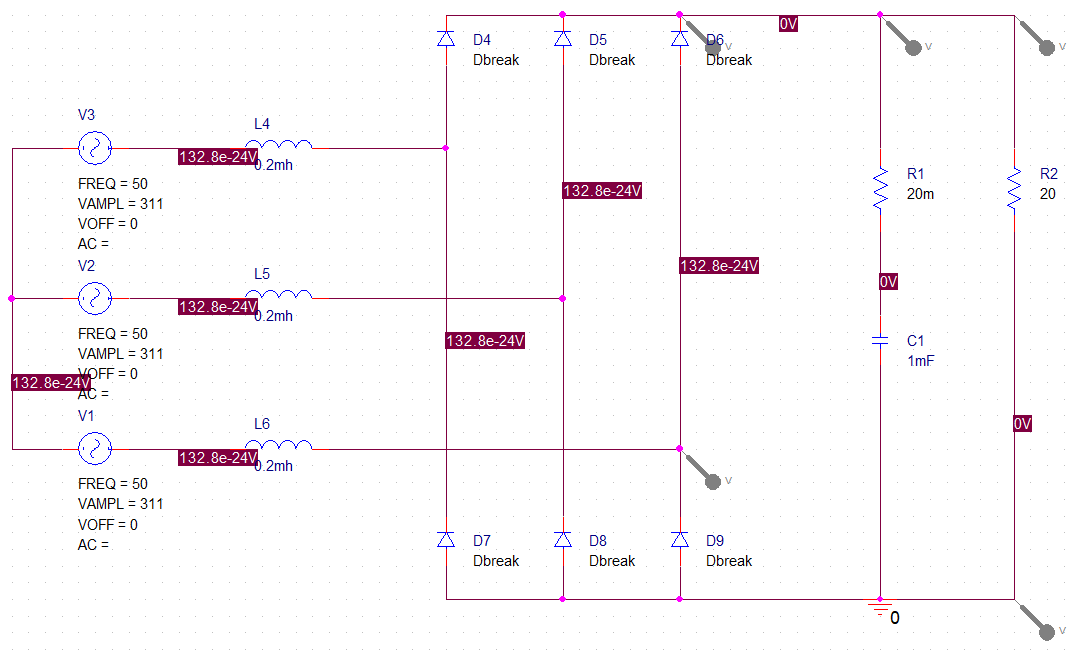
\includegraphics[scale=0.5]{cirp35.png}
            \caption{Circuito pagina 35.}
            \label{fig:cirp35}
        \end{figure}
        \begin{figure}[htbp]
            \centering
            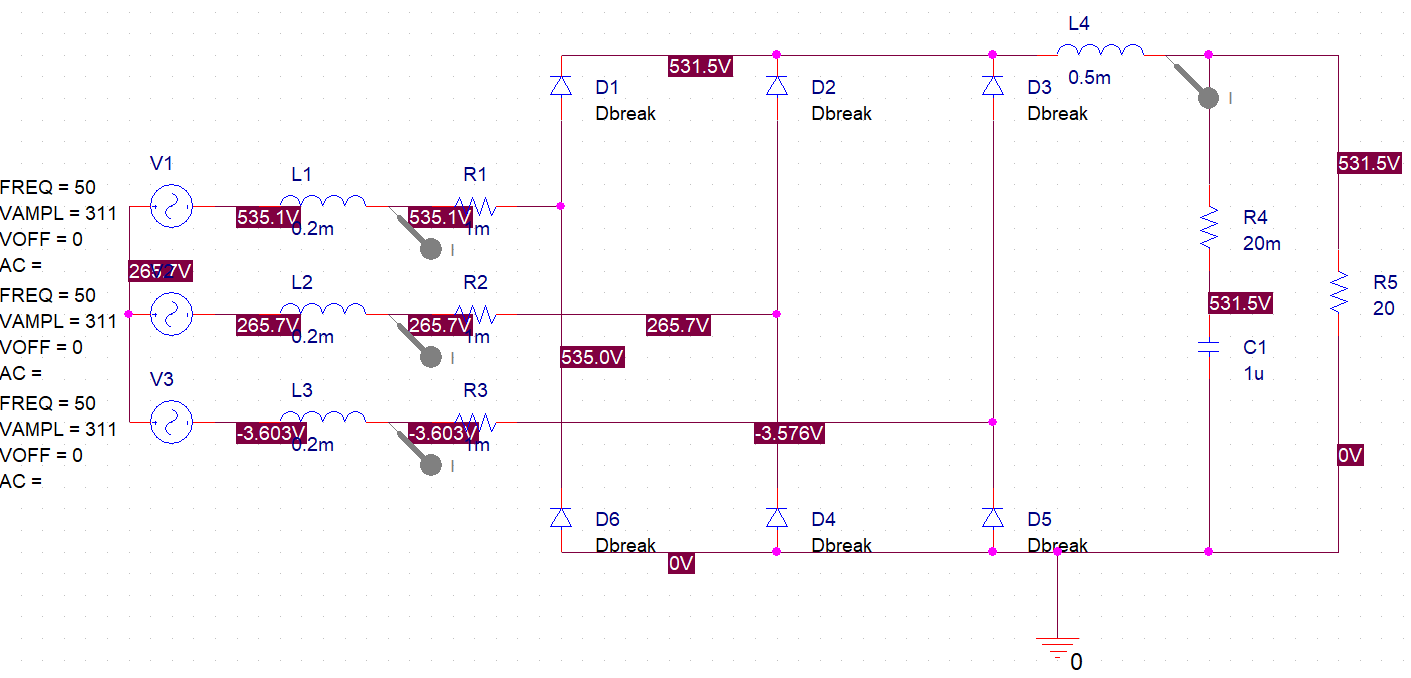
\includegraphics[scale=0.4]{cirp40.png}
            \caption{Circuito pagina 40.}
            \label{fig:cir40}
        \end{figure}
    \end{large}
    \newpage
    \vspace{1.2cm}

    \begin{LARGE}
     \textbf{Preguntas:}
     \end{LARGE}
 
 
 
 
 
 
 \begin{large}

\textbf{Actividad 1.1 Comprobar que el valor medio de la tensión en bornes
de la inductancia de carga es nulo en régimen permanente ¿Para qué
se debe cumplir esta condición?} \end{large}\\

    Bornes se define como la entrada y salida del circuito[los "bordes"] y el valor medio cuando la gráfica pasa por fase. Esta condición se debe cumplir para que la gráfica no pase por negativos

 \begin{large}

\textbf{Actividad 1.2 sustituir la resistencia de la carga por una fuente
de tensión continua de 150V. ¿De qué manera afecta esta modificación
al circuito?}\end{large}\\
Al sustituir la resistencia de carga por una fuente de tensión de 150V encontramos que la onda crece en el eje de las 'Y' manteniendose practicamente estable en 150V.\\
\begin{figure}[htbp]
    \centering
    \subfigure[Onda del circuito sin cambios.]{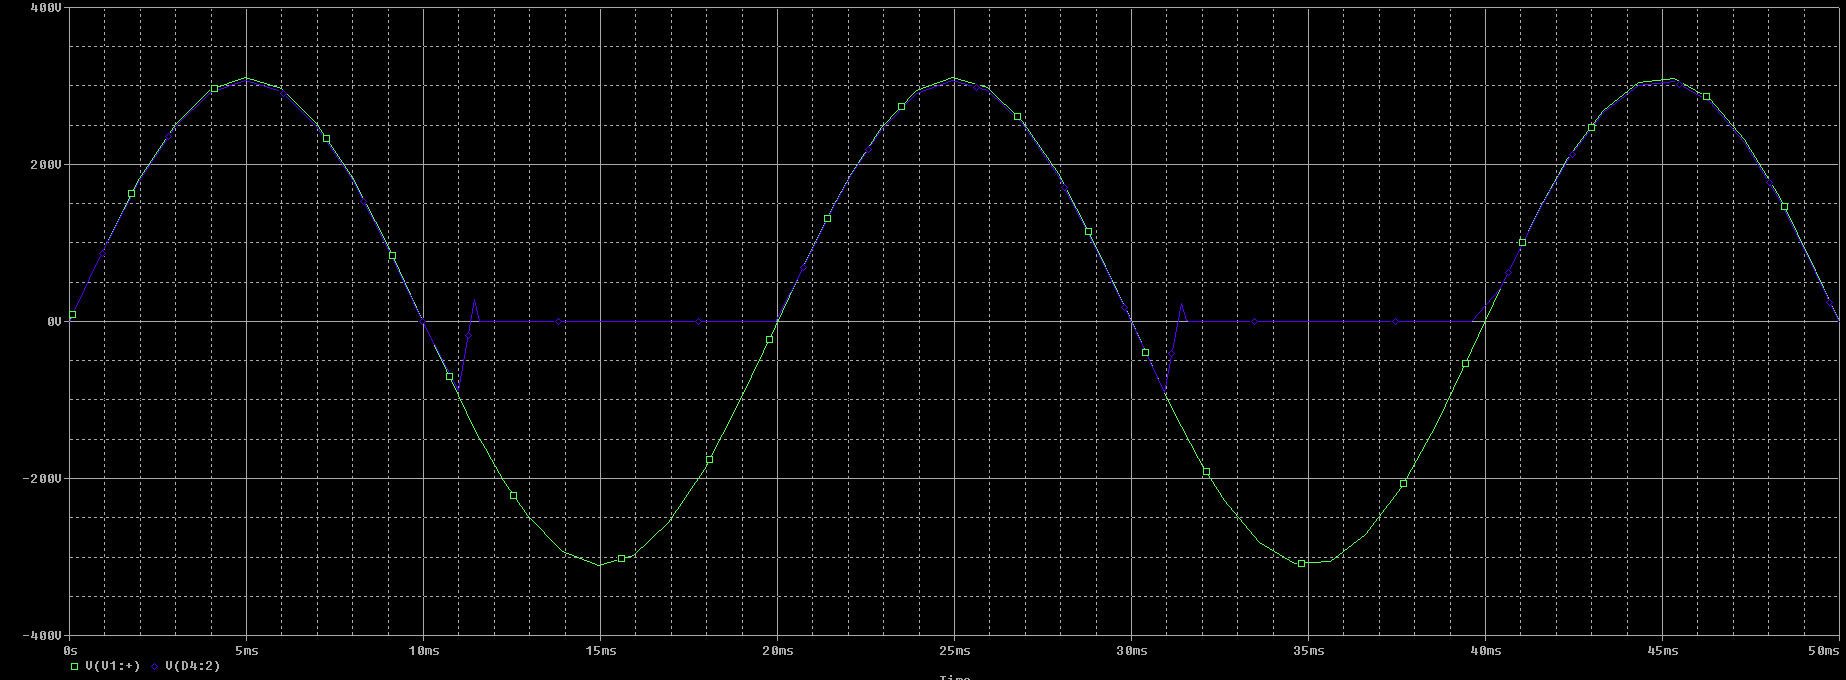
\includegraphics[scale=0.3]{ond1-1.png}}
    \subfigure[Onda con fuente de 150v]{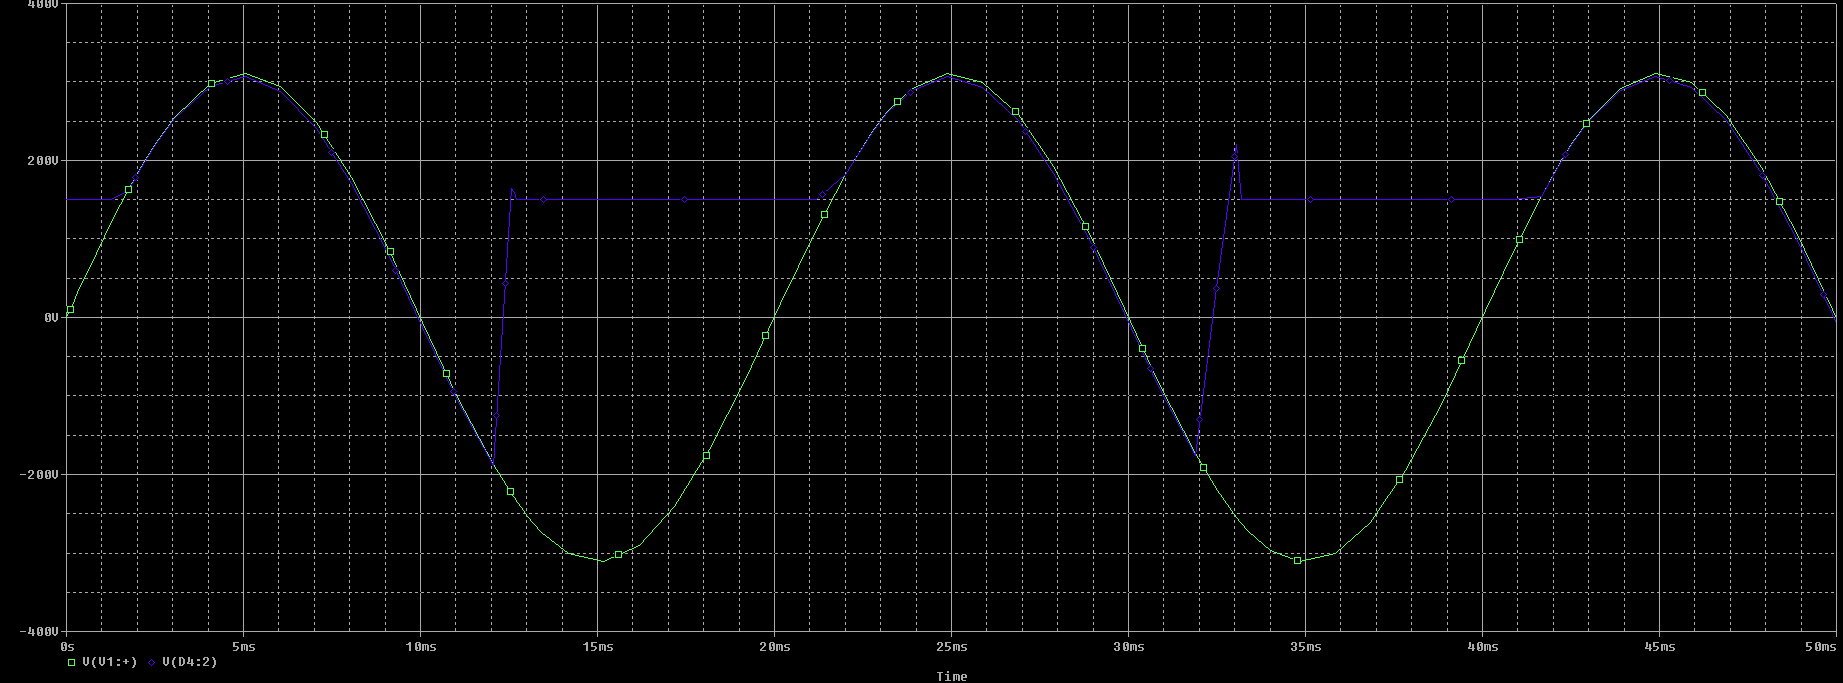
\includegraphics[scale=0.3]{ond1-2.png}}
    \caption{Ondas del circuito de la pagina 10.}
    \label{fig:my_labeeel}
\end{figure}
 \begin{large}

\textbf{Actividad 1.3 estudiar la influencia del valor de la capacidad de
filtrado sobre el rizado y el valor medio de la tensión aplicada a
la carga. Se recomienda efectuar un barrido paramétrico variando el
valor de CF desde 500uF hasta 10mF.} \end{large}\\
La tensión de carga está dada por el voltaje pico dos veces sobre pi, lo cual nos dice que según la onda que se obtenga con los capacitores y el 'smooth' que llegue a tener la onda será el valor afectado de voltaje pico y según sea el caso la onda crecerá o disminuirá.\\
A mayor capacitancia la onda sera mas estable tal y como lo muestran las ondas de la figura 14.\newpage
\begin{figure}[htb]
    \centering
    \subfigure[Rectificacion con 10mF]{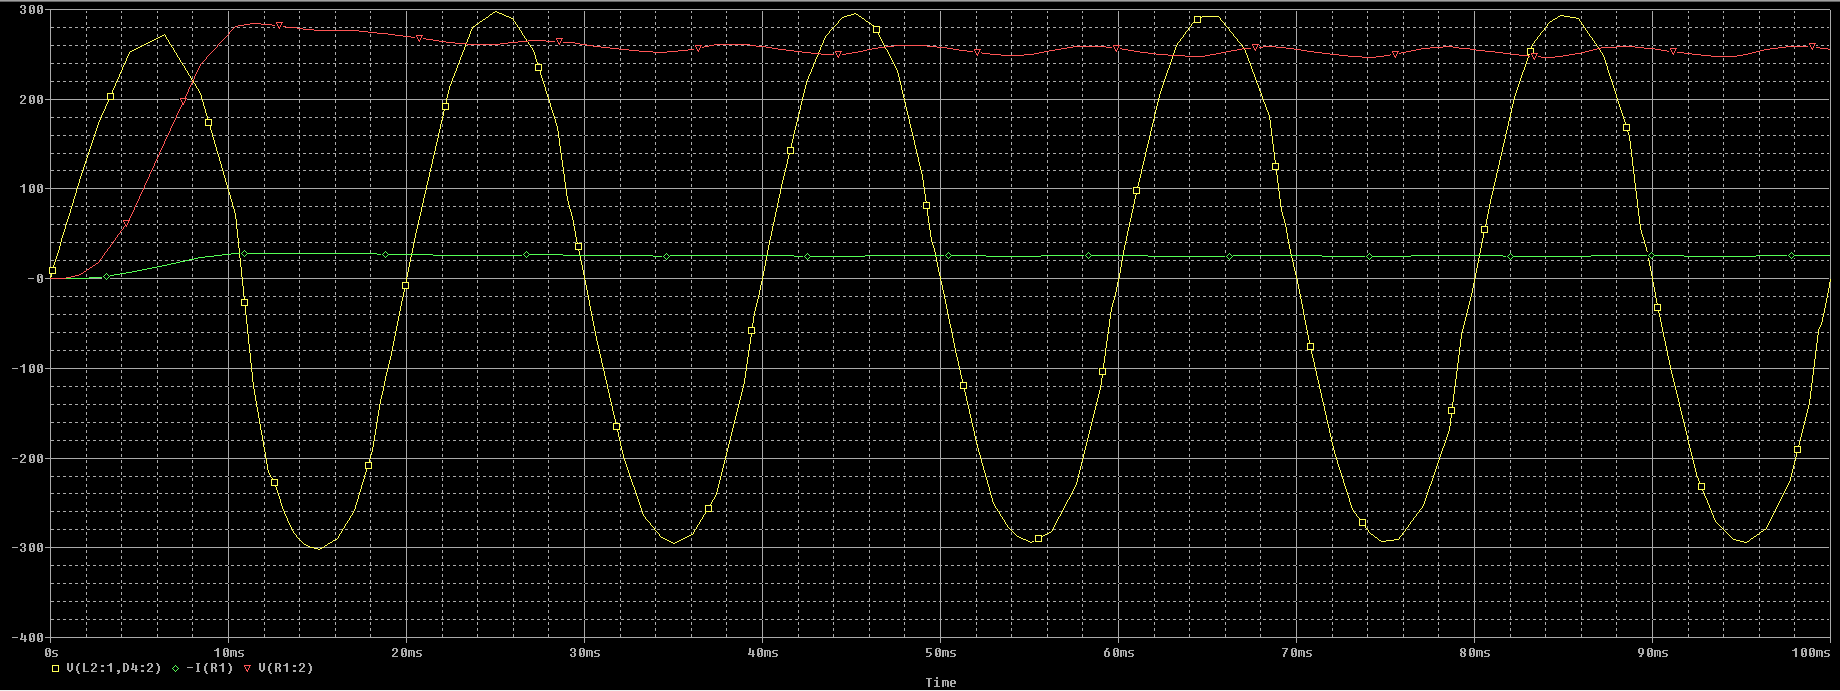
\includegraphics[scale=0.3]{ondcap10m.png}}
    \subfigure[Rectificacion con 500$\mu$F]{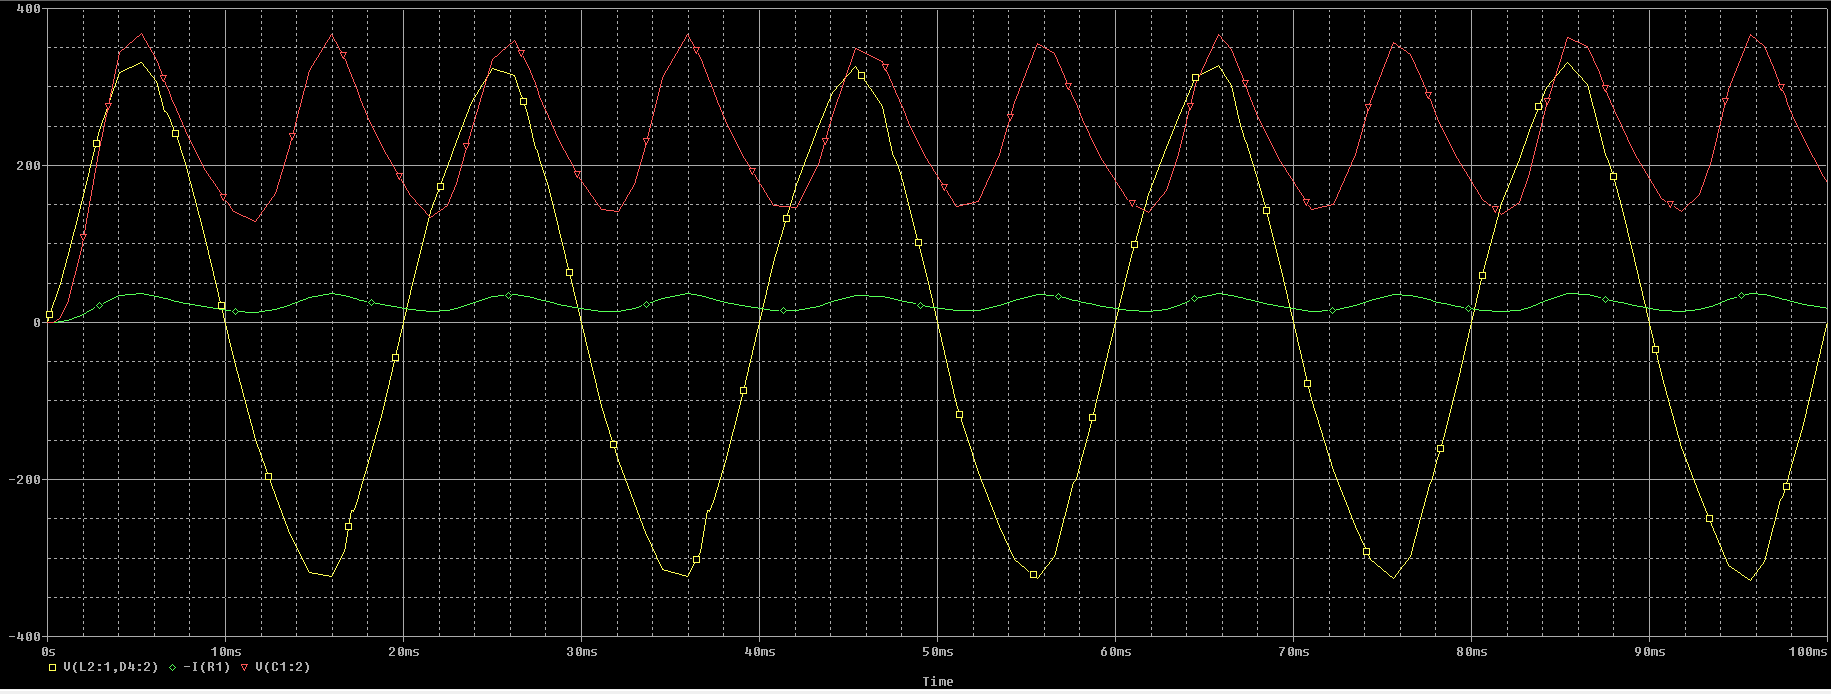
\includegraphics[scale=0.3]{ondacap500uf.png}}
    \caption{Comparativa de capacitancias}
    \label{fig:my_labeel}
\end{figure}
 \begin{large}

\textbf{Actividad 1.4 Estudiar cómo afecta al transitorio de carga del condensador
de filtro el valor de la capacidad, haciendo especial énfasis en la
corriente que circula por los diodos Pregunta actividad 1.4 ¿Qué medidas
pueden adoptarse para paliar los inconvenientes asociados a este transitorio?}\end{large}

\begin{large}
El periodo que dura la subida por parte del condencador afecta en la gráfica de manera que hace la onda mas "lisa" y ademas de esto para evitar paliar los dodos y el capacitor debemos utilizar corrientes que puedan soportar, evitando que se quemen o exploten.

\textbf{Actividad 1.4 Investigar la influencia de la inductancia de la red
(LR) sobre el factor de potencia del desplazamiento, la distorsión
armónica, el factor de potencia global y el rizado pico a pico de
la tensión de salida rectificada y filtrada.}\end{large}\\
El inductor[bobina] hace que la onda se haga con forma más senoidal que una onda descompuesta por varios elementos que se deben descomponer con el analisis de Fourier.\\
Al retrasar el flujo de la corriente la bobina reduce los armonicos y esto hace que el rizado sea mas facil de controlar por el capacitor.

 \begin{large}

\textbf{Actividad 1.5 repetir el estudio anterior modificando en esta ocasión
el valor de la capacidad del filtro CF.} \end{large}
la afectación que tiene en la onda es que la onda tiene más espacio entre 0 de eje 'x' y el espacio de la onda generada 
 \begin{large}

\textbf{Actividad 1.6 determinar la influencia de la inductancia de entrada
del rectificador (LR2), sobre el rizado de la tensión de salida, el
factor de potencia en la entrada y la distorsión de la tensión en
el PCC. ¿es conveniente añadir inductancias en la entrada del rectificador? }\end{large}
 \begin{large}\\
 Si lo es ya que esta reduce de buena manera el ruido de la saeñal pero si se pone demaciada habria perdida de potencia en el circuito.

\textbf{Actividad 1.7 obtener la forma de onda de la tensión y de la corriente
en los diodos del rectificador, determinando la tensión máxima que
deben soportar en inversa, así como el valor medio y el valor eficaz
de la corriente que conducen} \end{large}\\
Al ser un diodo ideal no existe tencion inversa antes del efecto avalancha.
\begin{figure}[htb]
    \centering
    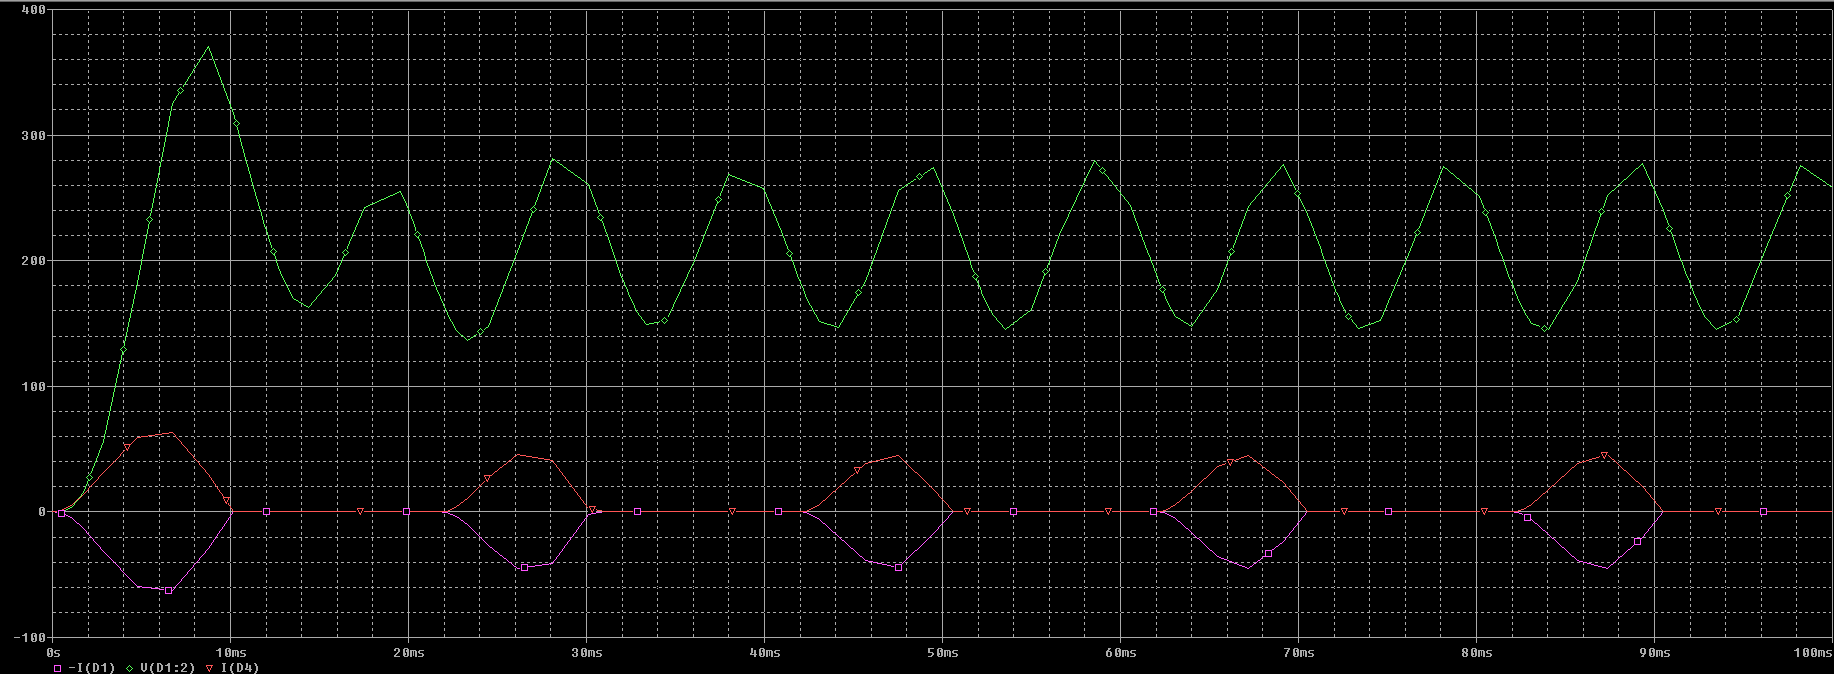
\includegraphics[scale=0.3]{ondadio.png}
    \caption{Graficas de intensidades de capacitor y voltaje de salida}
    \label{fig:cb15}
\end{figure}
 \begin{large}

\textbf{Actividad 1.8 calcula el factor de potencia del desplazamiento, la
distorsión armónica y el factor de potencia del rectificador duplicador
de tensión para varios regímenes de carga, comparando los resultados
con los obtenidos para el rectificador en puente.}\end{large}
 \begin{large}

\textbf{Actividad 1.9 Obtener las formas de onda de la corriente y de la tensión
en los diodos del rectificador duplicador de tensión. ¿Qué diferencia
se observan respecto al rectificador en fuente? }\end{large}
 \begin{large}
 \begin{figure}[htb]
     \centering
     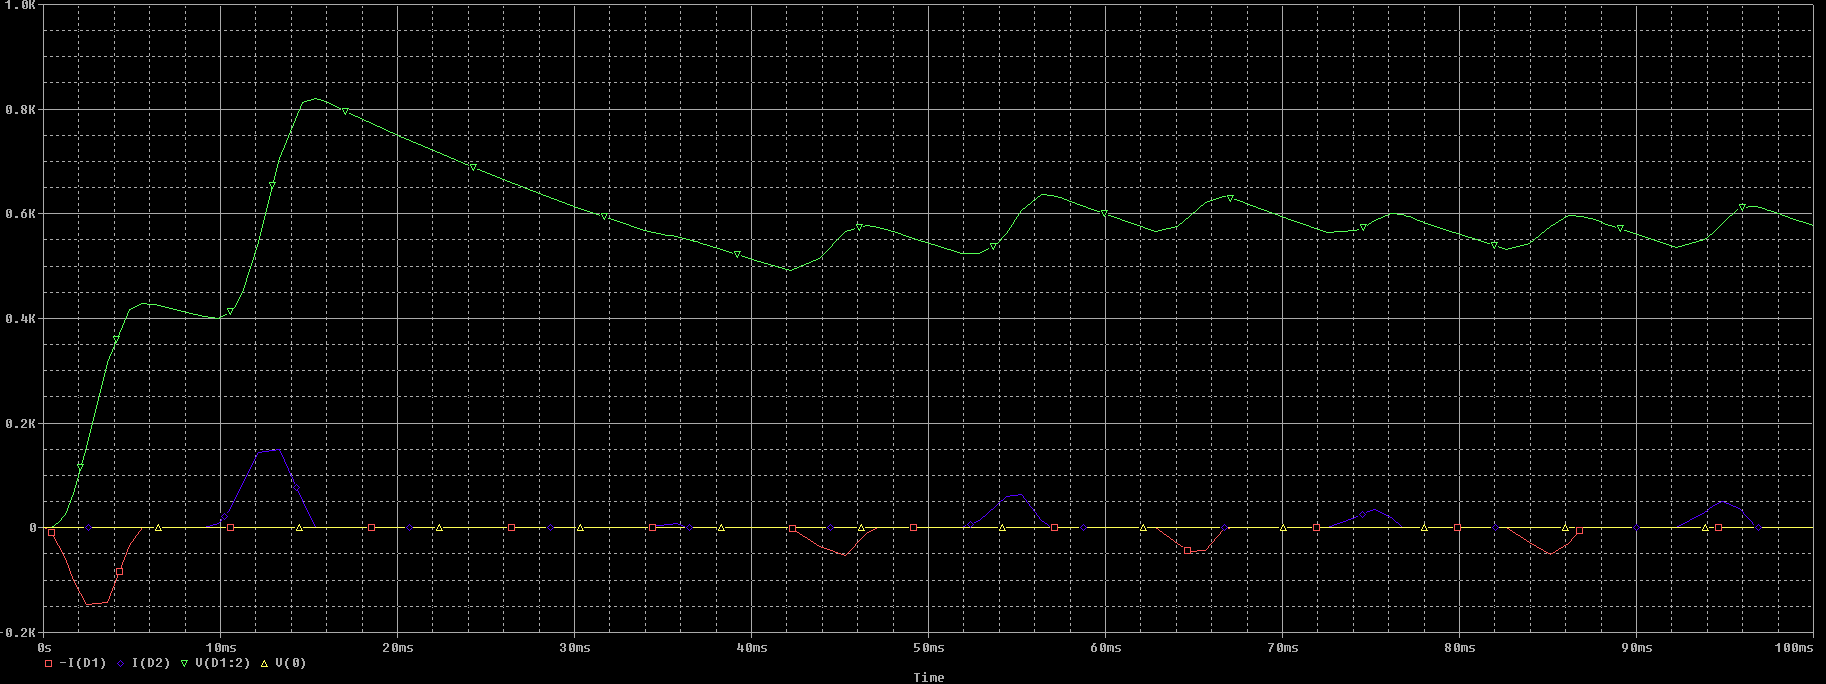
\includegraphics[scale=0.3]{ondacdup.png}
     \caption{Caption}
     \label{fig:my_label}
 \end{figure}

\textbf{Actividad 1.10 efectuar un análisis de Fourier sobre la corriente
que circula por el neutro, verificando que en el régimen permanente
se cumpla la siguiente relación. Siendo ILh el valor eficaz del armónico
de orden Lh de la corriente que circula por la línea.}\end{large} 
 \begin{large}
\[
I_{neutro(RMS)}=\sqrt{\sum_{h=3,6,9...}=(3*I_{Lh})^{2}}\approx3*I_{L3}
\]\end{large}
 \begin{large}

\textbf{Actividad 1.11 estudiar el efecto de desequilibrio de cargas eliminando
uno de los rectificadores ¿Qué sucede con la corriente de neutro en
esas condiciones?} \end{large}\\
Pareciera ser que nada importante ya que la onda se mantiene bastante similar a cuando lo tienia como se puede ver en la figura 17.\\
\begin{figure}[htb]
    \centering
    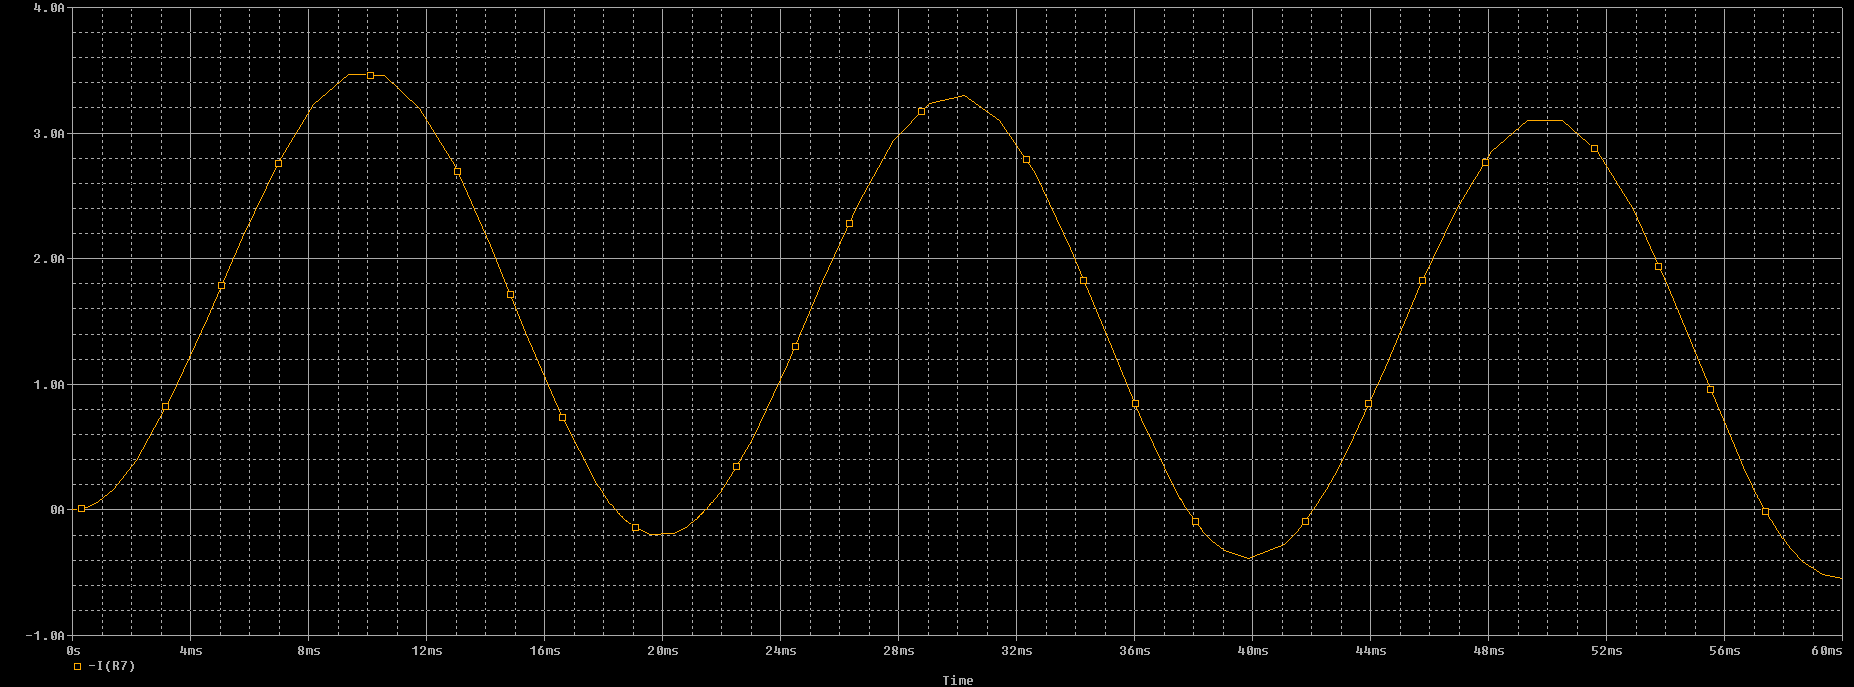
\includegraphics[scale=0.3]{intneu.png}
    \caption{Grafica de la intensidad en neutro}
    \label{fig:my_la45l}
\end{figure}
 \begin{large}

\textbf{Actividad 1.12 estudiar cómo evolucionan el rizado de la tensión de
salida, su valor medio y el factor de potencia del rectificador cuando
las inductancias de red varían de 0.1mH hasta 10mH }\end{large}
 \begin{large}

\textbf{Actividad 1.13 Repetir el estudio anterior variando esta vez el valor
de la resistencia de carga (10- 100 ohms)} \end{large}
 \begin{large}

\textbf{Actividad 1.14 obtener la forma de onda de la corriente que circula
por el condensador, determinando las pérdidas de potencia en el mismo,
teniendo en cuenta que.}\end{large}
 \begin{large}

\[
P_{Condensador}=R_{ESR}*I_{c(RMS)}
\]\end{large}

Siendo R(ESR) la resistencia equivalente en serie del condensador. 
 \begin{large}

\textbf{Actividad 1.15 analiza la evolución del valor medio y el rizado de
la tensión de salida para varios valores de la inductancia LF}\end{large}
 \begin{large}

\textbf{Actividad 1.16 Determina el factor de potencia y el valor medio de
la tensión del salida del rectificador cuando las inductancias de
red varían en un rango de 0.2mH a 10mH. Comparar con los resultados
del ejercicio anterior.} \end{large}
 \begin{large}

\textbf{Actividad 1.17 Obtener las formas de onda de la tensión y de la corriente
en uno de los diodos del rectificador, determinando los valores mas
significativos para la elección de dispositivos comerciales.} \end{large}
 \begin{large}

\textbf{Actividad 1.18 verificar que los resultados de la simulación corroboran
que la perdida de tensión media en la salida correspondiente a la
ec.(1.7)}.\end{large}
 \begin{large}

\[
\Delta V_{o}=\frac{\omega*L{r}}{2\pi}*I_{o}
\]\end{large}
 \begin{large}

\textbf{Actividad 1.19 verificar que los resultados de la simulación corroboran
que la perdida de tensión media en la salida del rectificador monofásico
corresponde a la ec(1.8).}\end{large}
 \begin{large}

\[
\Delta V_{o}=\frac{2\omega*L{r}}{\pi}*I_{o}
\]\end{large}
 \begin{large}

\textbf{Actividad 1.20 Estudiar el resto de las conmutaciones entre diodos
comprobando que cada una de ellas se produce la misma perdida de tensión
aplicada en la salida} \end{large}
 \begin{large}

\textbf{Actividad 1.21 Verificar que los resultados de la simulación corroboran
que la perdida de tensión media en la salida del rectificador trifásico
corresponde a la ec(1.10)}\end{large} \begin{large}

\[
\Delta V_{o}=\frac{3}{\pi}+\omega*L_{r}*I_{o}
\]
	\end{large}
    
    
    
    
    
    
    
    
    
    
    
    
    
    \begin{LARGE}
            \textbf{Conclusiones}\\
    \end{LARGE}
    
        \begin{large}    
		Conclusiòn Joel
       En un circuito rectificador es importante la adicion de reductores de ruido en la onda ya que fuera de pruebas de laboratorio la  onda nunca va a ser perfecta, siempre tendra ruido ya sea de interferencias exteriores o mismo desorden de la linea de alimentacion del circuito.\\
   		Conclusiòn Miguel
        Dentro de las afectaciones que se encuentran por parte de los componentes se puede encontrar una ventaja para crear ondas mas limpias y a la hora de hacer la descomposición de Furier es decir; tomar la onda y descomponerla en muchas ondas para que una tome coherencia, utilizando series matemáticas que muestren como dibujar cada onda.
        
        \end{large}

\end{document}